\chapter{Branch and Bound para PLI e Limitantes}

Resolvedores de PLI usam uma combinação do método de \textit{Branch and Bound} junto com a resolução de Programas Lineares (usando o Simplex por exemplo).

\section{Branch and Bound - Introdução}

A ideia básica é fazer uma busca exaustiva inteligente das soluções através de enumeração (branch) e poda (bound) das soluções ruins.

A enumeração das soluções é feita de acordo com os valores das variáveis inteiras. A ordem para se percorrer a árvore pode afetar a eficiência do algoritmo, normalmente percorre-se a árvore de acordo com o valor do limitante dual dos nós. O limitante dual indica que ``a partir desse ramo não é possíel obter uma solução melhor que esse valor''.

A poda dos ramos é feita de acordo com a viabilidade ou com a qualidade das soluções. A viabilidade é indicada pelas restrições do PLI. Para verificar se um nó é promissor ou não, vemos se o limitante dual do nó é pior que a melhor solução já encontrada $\to$ se o melhor do ramo for pior que o melhor que eu já tenho, ele não é promissor.

\section{Exemplo de Branch and Bound}

\begin{multicols}{2}
    \begin{itemize}
        \item Função objetivo: maximizar $x_1+2x_2$
        \item Restrições:
        \begin{itemize}
            \item $x_1 \leq 7,8\to$ \textcolor{blue}{$\alpha$}
            \item $x_2 \leq 5,9\to$ \textcolor{red}{$\beta$}
            \item $9x_1+16x_2\leq125\to$ \textcolor{green}{$\gamma$}
            \item $x_1,x_2\in\mathbb{Z}^+$
        \end{itemize}
    \end{itemize}

    \columnbreak

    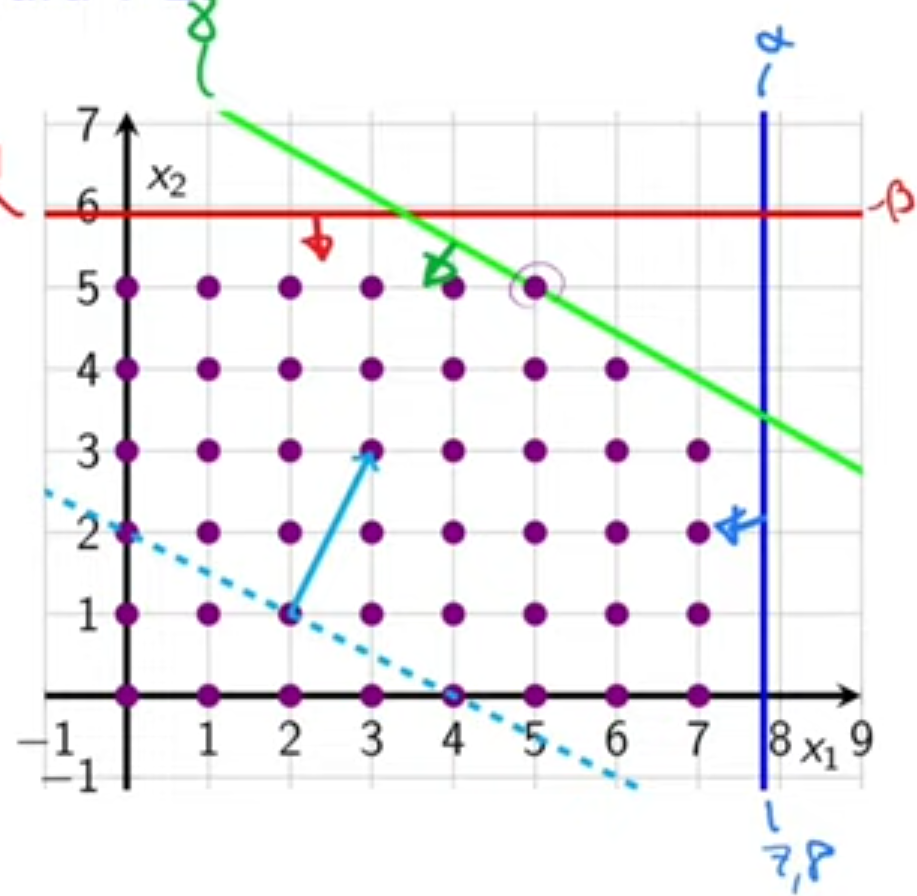
\includegraphics[width=.45\textwidth]{img/ex_branch_bound_1.png}
\end{multicols}

Para resolver o problema, primeiro relaxamos a integralidade do PLI ($x_1,x_2\in\mathbb{R}^+$) para encontrar o limitante dual das soluções através da solução de um problema de PL (através do Simplex, por exemplo).

Temos, por exemplo, como solução o ponto $(3,4; 5,9)$ com valor da função objetivo $15,2$. Com isso, a melhor solução (do PL) tem funçao objetivo $15,2$ como limitante dual (nenhuam solução do PLI vai ser melhor que isso).

Fazemos primeiro o \textit{branch} em torno da variáveis mais fracionária (em que o PL tem ``mais dúvida'').

\begin{center}
    \begin{tikzpicture}[every node/.style={fill=white}, n/.style={circle, draw}]
        \node[n] (1) at (0, 0) {15,2};
        \node[n] (2) [below left=of 1] {$x_1\leq3$};
        \node[n] (3) [below right=of 1] {$x_2\geq4$};

        \draw (1) edge (2);
        \draw (1) edge (3);
    \end{tikzpicture}
\end{center}

Agora temos dois subproblemas (dois novos polígonos) e repetimos o procedimento para cada novo subproblema (usamos o PL para calcular o limitante dual).

\begin{multicols}{2}

    \null \vfill
    \begin{center}
        \begin{tikzpicture}[every node/.style={fill=white}, n/.style={circle, draw}]
            \node[n] (1) at (0, 0) {15,2};
            \node[n, fill=violet!20] (2) [below left=of 1] {14,8};
            \node[n, fill=teal!20] (3) [below right=of 1] {15,125};
    
            \draw (1) edge node {$x_1\leq3$} (2);
            \draw (1) edge node {$x_1\geq4$} (3);
        \end{tikzpicture}
    \end{center}
    \vfill \null

    \columnbreak

    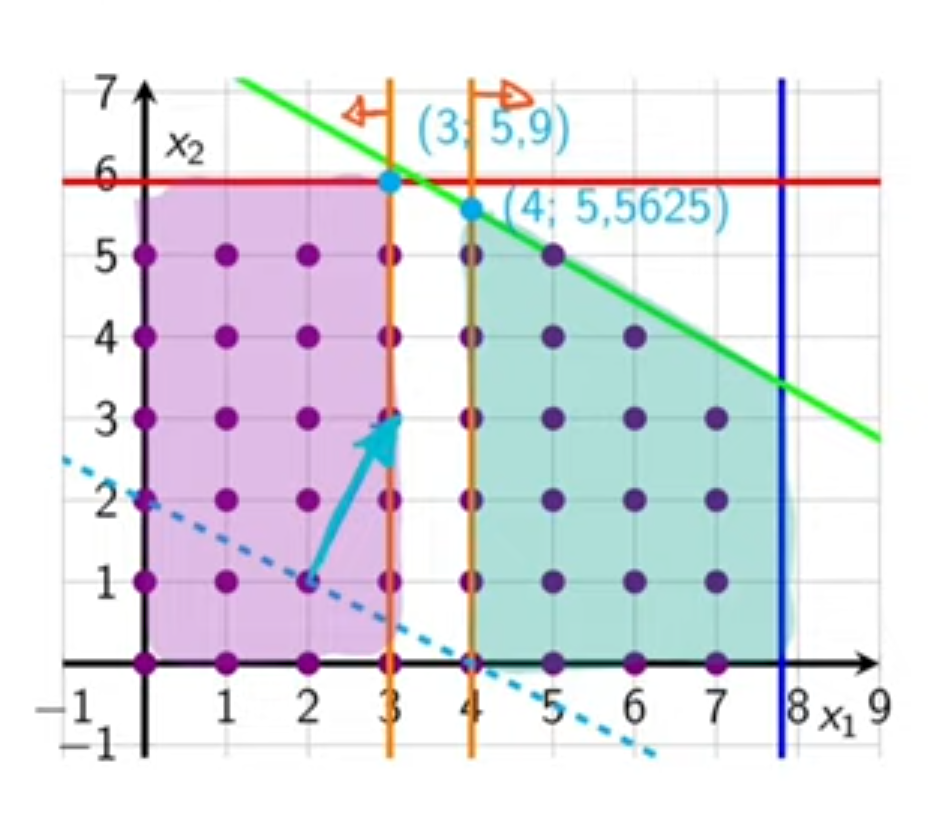
\includegraphics[width=.45\textwidth]{img/ex_branch_bound_2.png}
\end{multicols}

A partir daqui, podemos explorar seguindo aquele ramo que possui ``maior espaço para melhoria''. Ou seja, aquele cujo limitante dual esteja mais próximo do limitante dual original, nesse caso o ramo da direita. temos então como solução limitante $(4; 5,5625)$. $x_1$ não está fracionária, então fazemos a ramificação com a variável $x_2$.

\begin{center}
    \begin{tikzpicture}[every node/.style={fill=white}, n/.style={circle, draw}]
        \node[n] (1) at (0, 0) {15,2};
        \node[n] (2) [below left=of 1] {14,8};
        \node[n] (3) [below right=of 1] {15,125};
        \node[n] (4) [below left=of 3] {$x_2\leq5$};
        \node[n] (5) [below right=of 3] {$x_2\geq6$};

        \draw (1) edge node {$x_1\leq3$} (2);
        \draw (1) edge node {$x_1\geq4$} (3);
        \draw (3) edge (4);
        \draw (3) edge (5);
    \end{tikzpicture}
\end{center}

Com isso, temos:

\begin{multicols}{2}

    \null\vfill
    \begin{center}
        \begin{tikzpicture}[every node/.style={fill=white}, n/.style={circle, draw}]
            \node[n] (1) at (0, 0) {15,2};
            \node[forbidden sign, draw, fill=violet!20] (2) [below left=of 1] {14,8};
            \node[n] (3) [below right=of 1] {15,125};
            \node[n, fill=teal!20] (4) [below left=of 3] {15};
            \node[forbidden sign, draw] (5) [below right=of 3] {\phantom{X}};
    
            \draw (1) edge node {$x_1\leq3$} (2);
            \draw (1) edge node {$x_1\geq4$} (3);
            \draw (3) edge node {$x_2\leq5$} (4);
            \draw (3) edge node {$x_2\geq6$} (5);
        \end{tikzpicture}
    \end{center}
    \vfill\null

    \columnbreak

    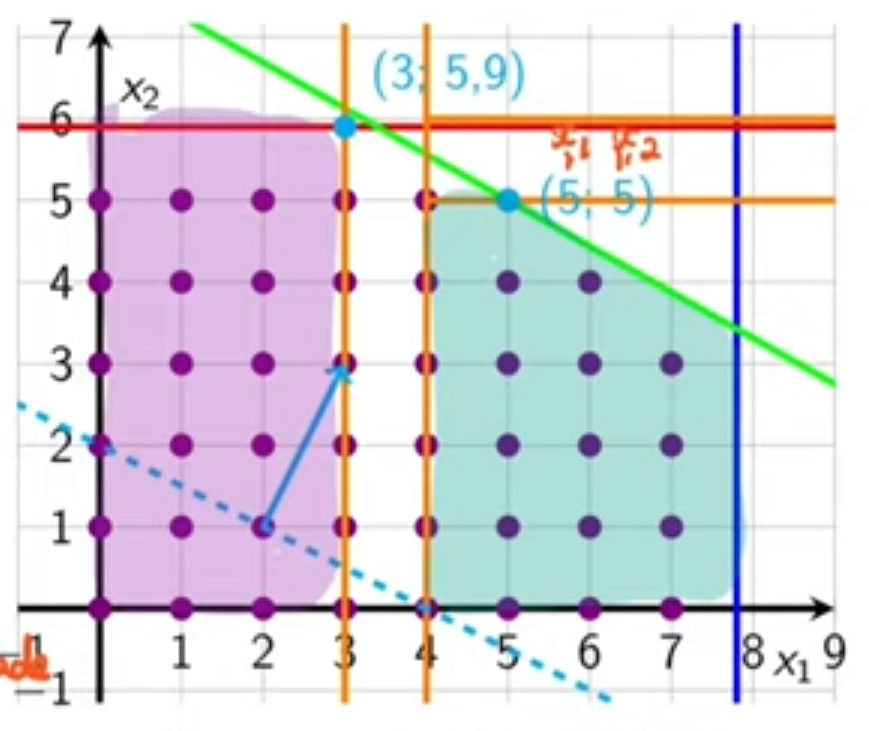
\includegraphics[width=.45\textwidth]{img/ex_branch_bound_3.png}
\end{multicols}

O ramo da direita não é mais explorado (é podado), pois temos uma inviabilidade, já que $x_2\geq6$ desrespeita a restrição $\beta$. Também não precisamos continuar explorando o ramo da esquerda, porque a solução do limitante dual já é inteira no ponto $(5; 5)$, então é a melhor solução inteira até o momento.

Deveríamos então continuar a explorar o subproblema em que $x_1\leq3$. Porém, sabemos que seu limitante dual é $14,8$, o que é menor que o valor da melhor solução inteira obtida (15), então não é necessário percorrer esse ramo, pois nunca terá uma solução melhor.

Como não temos mais nenhum nó ativo para ser percorrido, o algoritmo termina e temos como solução o ponto $(5; 5)$ com valor da função objetivo $15$.

\section{Pseudocódigo do Branch and Bound}

Enquanto houver \textbf{nós ativos}, escolher aquele com melhor (maximização/minimização) limitante dual.

\begin{itemize}
    \item Se o limitante dual for pior que a melhor solução já encontrada: eliminar o nó.
    \item Se a solução do PL desse nó for inteira, temos uma nova solução.
    \begin{itemize}
        \item Finalize o nó e atualize a melhor solução encontrada.
    \end{itemize}
    \item Caso contrário, ramifique o nó em torno da variável $x$ com valor $v$ mais fracionário (cuja parte decimal está mais perto de 0,5) na solução do PL.
    \begin{itemize}
        \item Crie dois subproblemas com $x\leq\lfloor v \rfloor$ e $x\geq\lceil v \rceil$
        \item Calcule o limitante dual do nó correspondente a cada subproblema
        \begin{itemize}
            \item Pode, por inviabilidade, podar aqueles que não tiverem solução
        \end{itemize}
    \end{itemize}
\end{itemize}

Antes de entrar no laço, calculamos o limitante dual do problema original e fazemos deste o primeiro nó.

\section{Problema da Mochila}

\begin{itemize}
    \item Variáveis: $x_i \in \{0,1\} \quad \forall i \in \{1,\dots,n\}$
    \item Função objetivo: $\max{\sum_{i=1}^nv_ix_i}$
    \item Restrição: $\sum_{i=1}^nw_ix_i\leq W$
\end{itemize}

Obtemos o PL, relaxando as restrições de integralidade $\to$ mochila fracionária.

O problema da mochila fracionária obtém a melhor solução através de um algoritmo guloso. Então podemos usar ele ao invés do Simplex.

\begin{example}
    \begin{itemize}
        \item $w_1=2\quad v_1=10\quad \frac{v_1}{w_1}=5$
        \item $w_2=3\quad v_2=21\quad \frac{v_2}{w_2}=7$
        \item $w_3=5\quad v_3=50\quad \frac{v_3}{w_2}=10$
        \item $w_4=7\quad v_4=51\quad \frac{v_4}{w_4}=8,5$
        \item $W = 7$
    \end{itemize}
\end{example}

Obtendo a melhor solução para o PL, usando o algoritmo guloso, temos que o limitante dual é: $v_3+\frac{2}{6}v_4=50+17=67$. A solução não é inteira, pois $x_4=\frac{1}{3}$. Ramificamos na variável mais fracionária ($x_4$).

\begin{example}
    \centering
    \begin{tikzpicture}[every node/.style={fill=white}, n/.style={ellipse, draw}]
        \node[n] (1) at (0, 0) {67};
        \node[n] (2) [below right=of 1] {$v_4+\frac{1}{5}v_3=61$};
        \node[n] (3) [below left=of 1] {$v_3+\frac{2}{3}v_2=64$};

        \draw (1) edge node {$x_4\geq1$} (2);
        \draw (1) edge node {$x_4\leq0$} (3);
    \end{tikzpicture}
\end{example}

Escolhemos o melhor limitante dual (como o problema é de maximização, pega-se o maior) e ramificamos de novo na variável mais fracionária ($x_2$). A restrição de que $x_4\leq 0$ continua valendo durante essa ramificação.

\begin{example}
    \centering
    \begin{tikzpicture}[every node/.style={fill=white}, n/.style={ellipse, draw}]
        \node[n] (1) at (0, 0) {67};
        \node[n] (2) [below right=of 1] {$61$};
        \node[n] (3) [below left=of 1] {$64$};
        \node[n] (4) [below right=of 3] {$v_2+\frac{4}{5}v_3=61$};
        \node[n] (5) [below left=of 3] {$v_3+v_1=60$};

        \draw (1) edge node {$x_4\geq1$} (2);
        \draw (1) edge node {$x_4\leq0$} (3);
        \draw (3) edge node {$x_2\geq1$} (4);
        \draw (3) edge node {$x_2\leq0$} (5);
    \end{tikzpicture}
\end{example}

Ramificamos novamente, o nó com limitante dual 61.

\begin{example}
    \centering
    \begin{tikzpicture}[every node/.style={fill=white}, n/.style={ellipse, draw}]
        \node[n] (1) at (0, 0) {67};
        \node[n] (2) [below right=of 1] {$61$};
        \node[n] (3) [below left=of 1] {$64$};
        \node[n] (4) [below right=of 3] {$61$};
        \node[n] (5) [below left=of 3] {$60$};
        \node[n] (6) [below right=of 4] {\sout{$w_2+w_3=8>7=W$}};
        \node[n] (7) [below left=of 4] {$v_2+v_1=31$};

        \draw (1) edge node {$x_4\geq1$} (2);
        \draw (1) edge node {$x_4\leq0$} (3);
        \draw (3) edge node {$x_2\geq1$} (4);
        \draw (3) edge node {$x_2\leq0$} (5);
        \draw (4) edge node {$x_3\geq1$} (6);
        \draw (4) edge node {$x_3\leq0$} (7);
    \end{tikzpicture}
\end{example}

Removemos o nó em que $x_3\geq1$ porque ao ter $x_2$ e $x_3$ inteiramente na mochila, o peso é excedido, então a solução não é viável. Seguimos ramificando no nó com o melhor limitante dual (61), em que $x_4\geq1$.

\begin{example}
    \centering
    \begin{tikzpicture}[every node/.style={fill=white}, n/.style={ellipse, draw}]
        \node[n] (1) at (0, 0) {67};
        \node[n] (2) [below right=of 1] {$61$};
        \node[n] (3) [below left=of 1] {$64$};
        \node[n] (4) [below right=of 3] {$61$};
        \node[n] (5) [below left=of 3] {$60$};
        \node[forbidden sign, draw, fill=red!20] (6) [below right=of 4] {\phantom{X}};
        \node[n] (7) [below left=of 4] {$31$};
        \node[n] (8) [right=2cm of 2] {\sout{$w_4 + w_3 = 11 > 7 = W$}};
        \node[n] (9) [below right=of 2] {$v_4+\frac{1}{3}v_2=51+7=58$};

        \draw (1) edge node {$x_4\geq1$} (2);
        \draw (1) edge node {$x_4\leq0$} (3);
        \draw (3) edge node {$x_2\geq1$} (4);
        \draw (3) edge node {$x_2\leq0$} (5);
        \draw (4) edge node {$x_3\geq1$} (6);
        \draw (4) edge node {$x_3\leq0$} (7);
        \draw (2) edge node {$x_3\geq1$} (8);
        \draw (2) edge node {$x_3\leq0$} (9);
    \end{tikzpicture}
\end{example}

Removemos mais um nó por inviabilidade. Continuamos explorando os nós ativos com maior limitante dual. Nesse caso, o de valor $60$, em que $x_4\leq0, x_2\leq0$. Nesse caso, a solução existente já é inteira. Com $x_3=1,x_1=1$ e limitante dual $60$. Portanto, essa é a melhor solução obtida até o momento, essa solução é chamada de \textbf{limitante primal}. Ele é desativado, por ser o melhor possível.

\begin{example}
    \centering
    \begin{tikzpicture}[every node/.style={fill=white}, n/.style={ellipse, draw}]
        \node[n] (1) at (0, 0) {67};
        \node[n] (2) [below right=of 1] {$61$};
        \node[n] (3) [below left=of 1] {$64$};
        \node[n] (4) [below right=of 3] {$61$};
        \node[n] (5) [below left=of 3, fill=green!20] {$60$};
        \node[forbidden sign, draw, fill=red!20] (6) [below right=of 4] {\phantom{X}};
        \node[n] (7) [below left=of 4] {$31$};
        \node[forbidden sign, draw, fill=red!20] (8) [right=2cm of 2] {\phantom{X}};
        \node[n] (9) [below right=of 2] {$58$};

        \draw (1) edge node {$x_4\geq1$} (2);
        \draw (1) edge node {$x_4\leq0$} (3);
        \draw (3) edge node {$x_2\geq1$} (4);
        \draw (3) edge node {$x_2\leq0$} (5);
        \draw (4) edge node {$x_3\geq1$} (6);
        \draw (4) edge node {$x_3\leq0$} (7);
        \draw (2) edge node {$x_3\geq1$} (8);
        \draw (2) edge node {$x_3\leq0$} (9);
    \end{tikzpicture}
\end{example}

Seguimos explorando os outros nós ativos em ordem. Seguindo o nó com limitante dual $58$. Como esse limitante é menor que o limitante primal encontrado anteriormente, o nó é apenas podado por limitante.

\begin{example}
    \centering
    \begin{tikzpicture}[every node/.style={fill=white}, n/.style={ellipse, draw}]
        \node[n] (1) at (0, 0) {67};
        \node[n] (2) [below right=of 1] {$61$};
        \node[n] (3) [below left=of 1] {$64$};
        \node[n] (4) [below right=of 3] {$61$};
        \node[n] (5) [below left=of 3, fill=green!20] {$60$};
        \node[forbidden sign, draw, fill=red!20] (6) [below right=of 4] {\phantom{X}};
        \node[n] (7) [below left=of 4] {$31$};
        \node[forbidden sign, draw, fill=red!20] (8) [right=2cm of 2] {\phantom{X}};
        \node[forbidden sign, draw, fill=red!20] (9) [below right=of 2] {$58$};

        \draw (1) edge node {$x_4\geq1$} (2);
        \draw (1) edge node {$x_4\leq0$} (3);
        \draw (3) edge node {$x_2\geq1$} (4);
        \draw (3) edge node {$x_2\leq0$} (5);
        \draw (4) edge node {$x_3\geq1$} (6);
        \draw (4) edge node {$x_3\leq0$} (7);
        \draw (2) edge node {$x_3\geq1$} (8);
        \draw (2) edge node {$x_3\leq0$} (9);
    \end{tikzpicture}
\end{example}

Em seguida, o nó com valor limitante 31 também é podado por limitante.

\begin{example}
    \centering
    \begin{tikzpicture}[every node/.style={fill=white}, n/.style={ellipse, draw}]
        \node[n] (1) at (0, 0) {67};
        \node[n] (2) [below right=of 1] {$61$};
        \node[n] (3) [below left=of 1] {$64$};
        \node[n] (4) [below right=of 3] {$61$};
        \node[n] (5) [below left=of 3, fill=green!20] {$60$};
        \node[forbidden sign, draw, fill=red!20] (6) [below right=of 4] {\phantom{X}};
        \node[forbidden sign, draw, fill=red!20] (7) [below left=of 4] {$31$};
        \node[forbidden sign, draw, fill=red!20] (8) [right=2cm of 2] {\phantom{X}};
        \node[forbidden sign, draw, fill=red!20] (9) [below right=of 2] {$58$};

        \draw (1) edge node {$x_4\geq1$} (2);
        \draw (1) edge node {$x_4\leq0$} (3);
        \draw (3) edge node {$x_2\geq1$} (4);
        \draw (3) edge node {$x_2\leq0$} (5);
        \draw (4) edge node {$x_3\geq1$} (6);
        \draw (4) edge node {$x_3\leq0$} (7);
        \draw (2) edge node {$x_3\geq1$} (8);
        \draw (2) edge node {$x_3\leq0$} (9);
    \end{tikzpicture}
\end{example}

\section{Eficiência do Branch and Bound}

A eficiência depende do número de podas, que depende de:

\begin{itemize}
    \item limitante primal (melhor solução encontrada até o momento)
    \item limitante dual (solução do PL relaxado para o nó sendo avaliado)
\end{itemize}

Então devemos encontrar \textbf{limitantes mais fortes}.

\textbf{Gap}: diferença entre o limitante primal e o limitante dual ``mais frouxo'' (melhor resultado) dos nós ativos. $\rightarrow$ \lstinline{RELATIVE_MIP_GAP}

\subsection{Fortalecendo limitantes primais}

Pode usar heurísticas e passar essa informação para o resolvedor de PLI. $\rightarrow$ \lstinline{SetHint}

Também é possível arrendondar a solução do PL para obter uma solução inteira. Tem que prestar atenção no sentido das desigualdades para saber se arredonda para cima ou para baixo. $\rightarrow$ Fazer isso abre mão de encontrar a solução ótima

É comum que resolvedores tenham como setar um \textit{callback} para chamar depois de encontrar a solução da relaxação. Pode usar isso para resolver o arredondamento. $\rightarrow$ Não tem no Or-tools, mas tem no Gurobi (pago)

Em geral, o valor de uma variável indica o quanto ela é ``interessante'' para a solução do problema.

\subsection{Fortalecendo limitantes duais}

O limitante dual é obtido da solução do PL vindo da relaxação. $\rightarrow$ Temos que melhorar a formulação do PL

Devemos encontrar \textbf{novas desigualdades} que \textbf{não} eliminam nenhuma solução \textbf{inteira} válida, mas que elimine soluções fracionárias da região viável. ``Diminui a área da região viável, aproximando as desigualdades do PL aos pontos inteiros''

Envoltória convexa, fecho convexo ou \textit{convex hull} $\rightarrow$ Menor conjunto convexo que possui todos os pontos de um conjunto. \textbf{Todo vértice é inteiro, desde que o conjunto só tenha pontos inteiros}.

Se encontrarmos a envoltória convexa do problema e executar a relaxação nesta área, vamos sempre obter a solução ótima. $\rightarrow$ Encontrar a envoltória convexa é NP-Difícil

\section{Problema do Conjunto Independente}

\begin{itemize}
    \item \textbf{Entrada:} grafo $G = (V, E)$
    \item \textbf{Soluções viáveis:} um conjunto $S \subseteq V$ tal que toda aresta $(u, v) \in E$ tem no máximo um extremo em $S$
    \item \textbf{Função objetivo:} tamanho de $S$
    \item \textbf{Objetivo:} encontrar solução de valor máximo
\end{itemize}

\subsection{Formulação em PLI para o Conjunto Independente}

\begin{itemize}
    \item Variáveis: $x_u \in \{0, 1\} \quad \forall u \in V$
    \item Função objetivo: $\max \sum_{u \in V}x_u$
    \item Restrição: $x_u + x_v \leq 1 \quad \forall (u, v) \in E$
\end{itemize}

Na relaxação: $0 \leq x_u \leq 1$.

\begin{example}
    \begin{center}
        \begin{tikzpicture}[every node/.style={fill=white}, n/.style={circle, draw}]
            \node[n] (a) at (0, 0) {a};
            \node[n] (b) [below right=of a] {b};
            \node[n] (c) [below left=of a] {c};

            \draw (a) edge (b);
            \draw (a) edge (c);
            \draw (c) edge (b);
        \end{tikzpicture}
    \end{center}
\end{example}

Se no exemplo $x_a = 0,5; x_b=0,5; x_c=0,5$. O limitante dual é $1,5$, enquanto o limitante primal é $1,0$.

Sabendo que o grafo é um triângulo (as arestas vão ter que ficar sozinhas em $S$), podemos criar uma outra restrição $x_a + x_b + x_c \leq 1$. Essa restrição não elimina nenhuma solução inteira, mas melhora as soluções do PL relaxado.

Isso pode servir a qualquer subgrafo completo (todos os nós conectados). $\rightarrow$ Clique
